\chapter{Estado del arte}
\label{estado.arte}

\section{Impresoras 3D}
\label{arte_immpresoras}

En los últimos años ha tenido un gran auge las denominadas impresoras 3D. Máquinas capaces de crear un objeto físico de cero mediante un proceso de fabricación aditiva. Este tipo de fabricación está siendo una nueva revolución, de igual manera que pasó hace unos años con la conocida Web2.0, en la que el usuario era capaz de generar contenido para la propia página. Con la fabricación aditiva, pasaremos de la fabricación 1.0 (Produción de objetos físicos por grandes empresas y expertos) a la fabricación 2.0 (producción de los objetos por el cliente final).\cite{additive}\\

La fabricación aditiva es una colección de procesos que unen materiales para crear objetos fisicos en 3D directamente desde un diseño en ordenador. Estos procesos, se caracterizan en que van añadiendo distintas capas, que es todo lo contrario al mecanizado, en la que se conforma la pieza por eliminación de material, ya sea por arranque de viruta o por abrasión.\\

Una de las ventajas de la fabricación aditiva es su rápidez \cite{additivevssubtractive}, dependiendo de la complejidad de la pieza puede suponer un par de horas de fabricación, frente a una jornada completa de trabajo con las máquinas de mecanizado. Por ello, también se conocen a este tipo de máquinas, como máquinas de prototipado rápido.\\

    \begin{figure}[H]
            \centering
            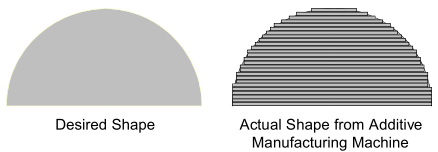
\includegraphics[width=0.6\textwidth]{images/aproximacion_am.png}
            \caption{Aproximación de una pieza con fabricación aditiva. Fuente \cite{additive}}
            \label{fig:approach_am}
    \end{figure}

Antiguamente, cuando sólo las grandes empresas disponian de ordenadores y se quería hacer algún tipo de cálculo numérico o tratamiento de información, era necesario ir a los centros de cálculos con los datos requeridos, para que, despues de días o incluso semanas, obtener nuestros resultados y en el mejor de los casos, haber realizado correctamente el ensayo y no tener que volver a repetirlos, si los resultados no eran los deseados, se debería volver a repetir la operación. Con la fabricación de las piezas pasa algo similar. En el caso de que quisieramos diseñar alguna pieza para cubrir nuestras necesidades, debíamos acudir a empresas que dispusieran de las máquinas necesarias para tratar los materiales, y pasado cierto tiempo, tendríamos la pieza en nuestras manos. Una vez en nuestro poder, deberíamos comprobar que la pieza cumple con nuestras especificaciones y ver que no nos equivocarámos a la hora de tomar alguna medida y saber las tolerancias de la máquina. Gracias a la tecnología aditiva, el tiempo se ha acortado, y como veremos más adelante, a día de hoy, no es necesario acudir a ninguna empresa para poder realizar nuestras propias piezas.\\

La tecnología aditiva lleva muchos años usandose y sin embargo no ha sufrido muchos cambios desde que empresas como 3Dsystems, Stratatasys o incluso el MIT, la usaran a medidados de los años 80. A pesar de ello, no ha sido hasta hace unos pocos años (2009) cuando la tecnología ha llegado al público en general. Se debe a que el funcionamiento de este tipo de tecnologías estaban protegidas por patentes. La principal patente \cite{crump1992apparatus} es la que desarrolló \textbf{S. Scott Crump} co-fundador de Stratasys, la cual expiro en 2009 y permitió que pudiera extenderse el uso de esta tecnología.\\

\section{Tecnologías de fabricación aditiva}

Dentro de la fabricación aditiva, existen varios modelos de máquinas, en las que el principio de funcionamiento es el mismo, pero la forma de materializar la pieza final son distintas.

Algunas de las tecnologías más usadas son las siguientes:


\begin{table}[H]
\centering
\begin{tabular}{| >{\centering\arraybackslash}m{8cm} | >{\centering\arraybackslash}m{7cm}|}
    \hline
    \multirow{5}{9cm}{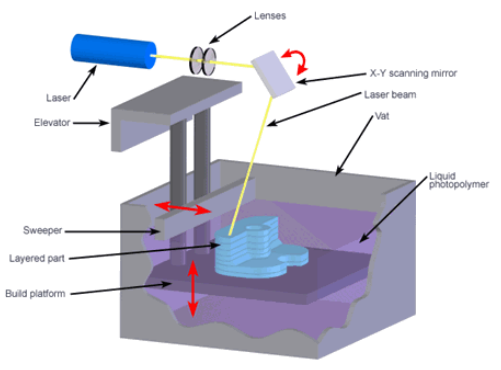
\includegraphics[width=0.4\textwidth]{./images/SLA.png}}\\
    & \textbf{Estereolitografía (SLA)}\\
    & Considerada la primera técnica de fabricación aditiva.\\
    & Fue patentada en 1986 y fabricada por 3d Systems en 1987.\\
    & El prinipio de funcionamiento es la polimerización de una resina fotucable.\\
    & Puede alcanzar un espesor de capa de $100\mu m$.\\
    \hline
    \multirow{5}{9cm}{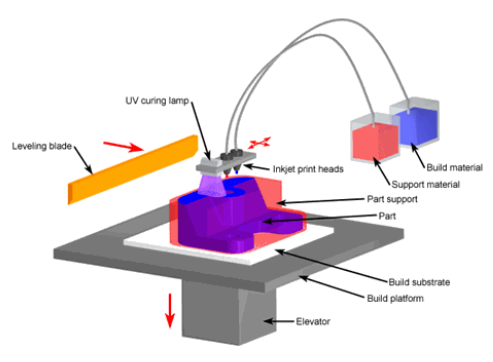
\includegraphics[width=0.4\textwidth]{./images/polyjet.png}}\\
    & \textbf{Polyjet}\\
    & De la empresa Israelí Objet.\\
    & Patentada a finales de los 90\\
    & Resina fotocurable de base acrilato.\\
    & Necesita soportes.\\
    \hline
    \multirow{5}{9cm}{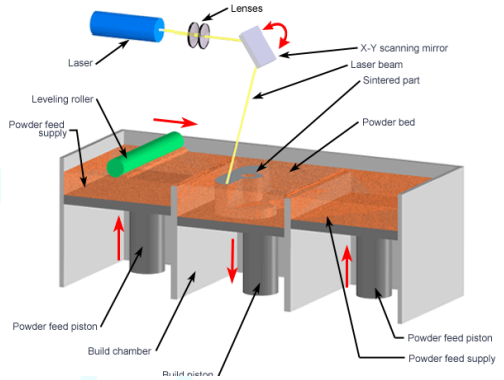
\includegraphics[width=0.4\textwidth]{./images/sls.png}}\\
    & \textbf{Selective Lase Sintering (SLS)}\\
    & Patentada en 1979.\\
    & Procesado de polímeros, metales y cerámicos.\\
    & Puede alcanzar un espesor de capa de $100\mu m$.\\
    & Necesidad de recubrimiento en maetales y cerámicos para ser sinterizados.\\
    \hline
    \multirow{4}{9cm}{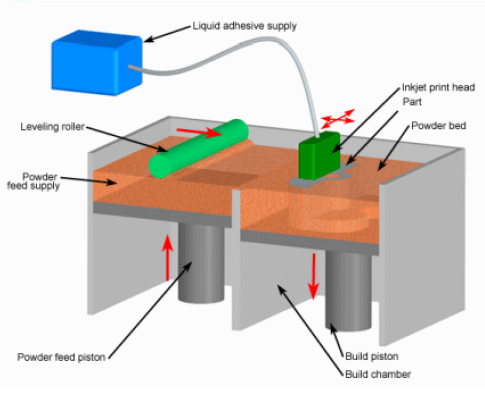
\includegraphics[width=0.4\textwidth]{./images/3d_mit.png}}\\
    & \textbf{Three Dimensional Printing}\\
    & Patentada en el MIT.\\
    & Para mezclas de cerámicos.\\
    & Se usa en modelos y maquetas.\\
    \hline
    \multirow{4}{9cm}{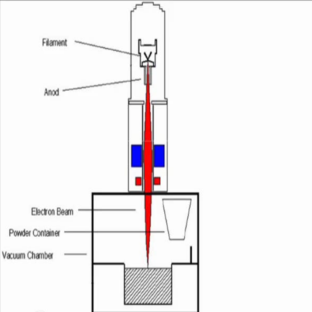
\includegraphics[width=0.4\textwidth]{./images/ebm.png}}\\
    & \textbf{Electron Beam Melting (EBM)}\\
    & Fabricada y comercializada por Arcam (1997).\\
    & Funde polvo metálico de varias aleaciones, incluyendo las de Titanio.\\
    & Alta velocidad de producción por la potencia del haz de electrones y la posibilidad de guiarlo cambiando el campo magnético a través del cual pasa el haz.\\
    \hline
    \multirow{6}{9cm}{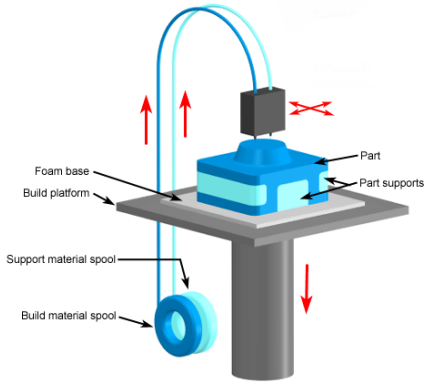
\includegraphics[width=0.4\textwidth]{./images/fdm.png}}\\
    & \textbf{Fused Deposition Modelling (FDM)}\\
    & Comercializada por Stratasys en 1991.\\
    & Extrusión de filamento (Polímeros).\\
    & Tecnológia más extendida\\
    & Necesita soportes.\\
    & Varios tipos de termoplásticos.\\



\end{tabular}
\caption{Tecnologicas de fabricación aditiva. Fuente \cite{FabricacionAditiva}.}
\label{tabla:autores}
\end{table}

Sin embargo la que más se ha popularizado en la sociedad es la de materíal extruido ya que es la tecnología más sencilla de realizar de manera doméstica. En el siguiente capitulo se detallará en profundidad su funcionamiento, ya que es la tecnología que va abordar este proyecto.

\section{Fabricación de modelado por deposición fundido}
La fabricación de modelado por deposición fundido (\textbf{FDM\textregistered} en inglés) es la tecnología aditiva que más se ha popularizado en los últimos años. Aunque estas siglas están registradas por la empresa Stratasys Inc. ya que su co-fundador,  \textbf{S. Scott Crump} fué quien desarrollo está tecnología, y poseedor de la patente en la que se detalla su funcionamiento \cite{crump1992apparatus}. Por ello, se usa el término equivalente, fabricación con filamento fundido (\textbf{FFF}).\\  
    
    \begin{figure}[H]
            \centering
            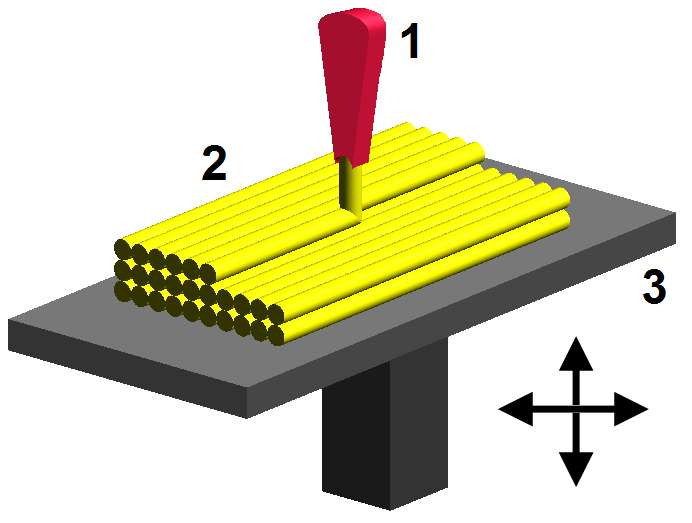
\includegraphics[width=0.4\textwidth]{images/FDM_by_Zureks.png}
            \caption{Principio de la fabricación con filamento fundido. Fuente \cite{fundamentoFDM}}
            \label{fig:impr_fdm}
    \end{figure}

En la imagen \ref{fig:impr_fdm} podemos ver en detalle el principio de funcionamiento de este tipo de impresoras. La máquina dispone de un elemento fusor (1), que está por encima de la temperatura de transición vítrea del polímero, haciendo que entre en un estado viscoso y maleable. El fusor deposita el polímero (2) en distintos niveles sobre una superficie plana (3) a la vez que se desplaza en los tres ejes cartesianos (X,Y,Z), de este modo, la pieza es creada con el filamento que solidifica al salir del fusor.\\

    \begin{figure}[H]
            \centering
            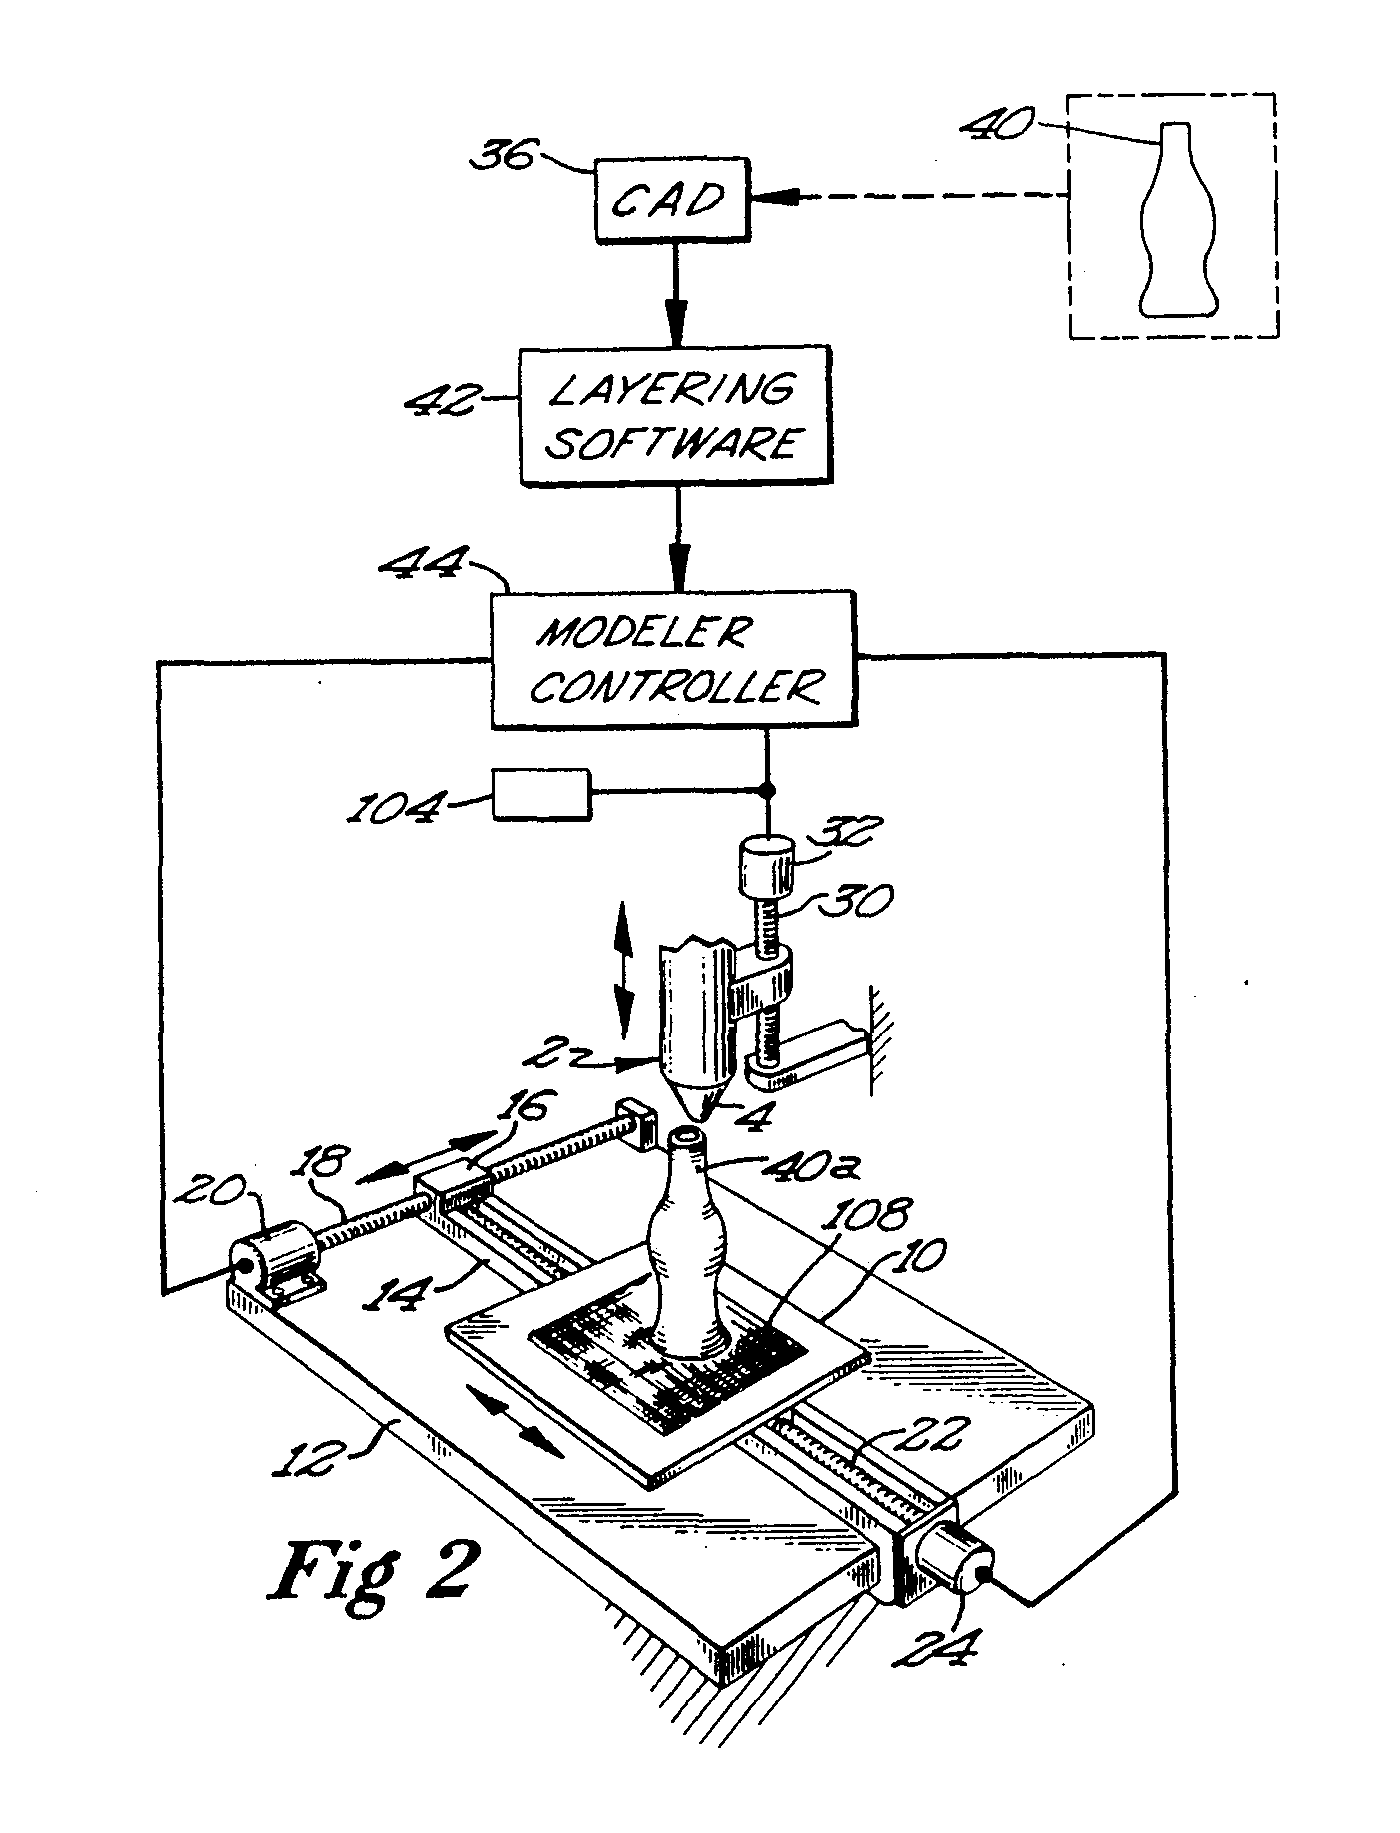
\includegraphics[width=0.6\textwidth]{images/estado.arte/US5340433-2.png}
            \caption{Esquema de la patente de S. Scott Crump. Fuente  \cite{crump1992apparatus}}
            \label{fig:impr_patente_sistema}
    \end{figure}

Este sistema de fabricación, tiene tres pasos definidos:
\begin{itemize}
    \item \textbf{Pre-procesado:} Un software especial lamina en capas y calcula las trayectorias necesarias para crear el objeto que queremos fabricar.
    \item \textbf{Producción:} La impresora 3D calienta el termoplástico hasta alcanzar un estado viscoso y maleable y lo va depositando en capas muy finas siguiendo las trayectorias anteriormente calculadas por el software. En los sitios en los que es necesario un soporte, la impresora pone material que posteriormente será quitado de la pieza final.
    \item \textbf{Post-procesado:} Una vez que la impresora termina, la pieza será usable. En caso de haber puesto material, el usuario deberá removerlo antes de poder dar la pieza por terminada.
\end{itemize}

Según explica stratasys en su págnia web \cite{FDMTechnology}, la tecnología FFF tiene varios beneficios que la hacen idonea para fabricar:
\begin{itemize}
    \item La tecnología es limpia y facil de usar por el usuario.
    \item Los termoplásticos usados son estables mecanicamente y con el medio ambiente.
    \item Formas complejas que con otra tecnología serían costosas de fabricar, con FFF son mucho más practicas de realizar.
\end{itemize}

El motivo de su crecimiento ha sido gracias a que en 2009 expiró de la patente de S. Scott Crump \cite{crump1992apparatus} y se ha dado la posibilidad de que surgan unos modelos \textit{Do It Yourself} (DIY), de tal manera que uno mismo es capaz de fabricarse una impresora con materiales facilmente disponibles, reduciendo así el precio de la máquina. También se ha generado una gran comunidad de usuarios en donde se comparte conocimientos y vivencias de los usuarios, haciendo más fácil la iniciativa a que la gente construya sus propias impresoras. 

\subsection{Materiales usados en impresión 3D}
\label{impreso_materiales}
En la actualidad hay multitud de materiales que se pueden usar en las impresoras 3D. Siendo la mayoría de ellos polímeros termoplásticos, ya que si se les aplica una temperatura alta se vuelven deformables y al enfriarlos, pasando por un estado de transición vítrea, se endurecen.\\

Algunos materiales que se usan son:
\begin{itemize}
    \item \textbf{ABS} o acrilonitrilo butadieno estireno.
    \item \textbf{PLA} o poliácido láctico.
    \item \textbf{PVA} o alcohol de polivinilo.
    \item \textbf{NYLON.}
\end{itemize}

Todos ellos tienen características que hacen idóneo su uso en diferentes campos. Por ejemplo, el ABS tiene unas propiedades mecánicas mejores que el PLA. Por ello, en función de la utilidad que se vaya a dar a la pieza final, será recomendable usar un polímero u otro. Todos estos consumibles comparten la característica de como se distribuyen. El polímero es introducido en el fusor de la impresora en forma de filamento para de ese modo conseguir un hilo continuo durante la impresión.\\

Por ello, el método de fabricación del consumible es la extrusión, ya que es el método que mejor se amolda para crear objetos con una sección transversal definida y fija.

\section{Extrusión de polímeros}
\label{arte_extrusion}
La extrusión de polímeros es un proceso industrial de fabricación, en el cual se hace pasar por un troquel (también denominado dado) la matería prima previamente prensada y calentada. El proceso de prensado y calentamiento, se hace en una cámara, que contiene un tornillo sin fin el cual gira concentricamente y es alimentado por una tolva. Al hacer pasar el polímero por el troquel, se consigue un objeto con un perfil constante y una longitud variable, pudiendo llegar a ser de centímetros, o en algunos casos de metros.

\begin{figure}[H]
        \centering
        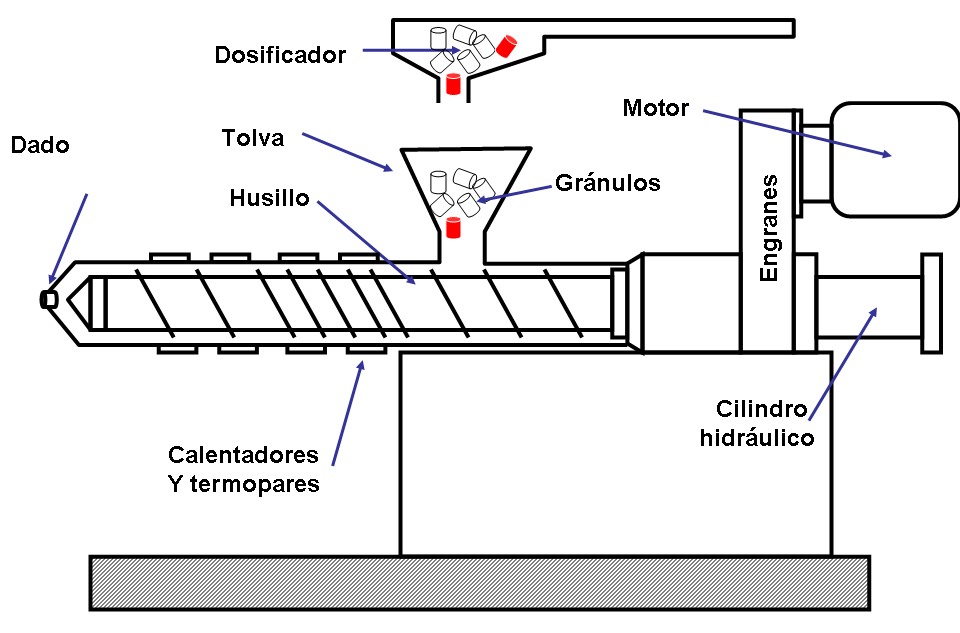
\includegraphics[width=0.6\textwidth]{images/extrusor.png}
        \caption{Esquema básico de una extrusora. Fuente \cite{disenoextrusor}}
        \label{fig:estado_extrusora}
\end{figure}

Las principales variables de control que inluyen en el acabado del producto final, son la velocidad de extrusión y la temperatura del cilindro hidráulico afectando estos en la calidad final del producto.\\

La velocidad influye directamente en el caudal de producción de la máquina. Teóricamente, al incrementar la velocidad del husillo, obtendríamos una mayor producción en la línea, por contra repercute en la calidad final haciendo que la mezcla del producto no sea homogena y llegando a producirse la denominada fractura del polímero fundido, que es debido a la fricción que sufre el polímero al salir por el dado.\\

La temperatura por contra, influye en la viscosidad del polímero, este parámetro repercute directamente en la resistencia al fundido. Lo cual es bastante importante, por que en el caso que nos ocupa, el  material obtenido será posteriormente fundido en una impresora 3D.\\

En la imagens \ref{fig:estado_extrusora} podemos observar los distintos elementos que conforman la extrusora:
\begin{itemize}
    \item \textbf{Dosificador:} es el encargado de suministrar el polímero, normalmente en forma de granza, a la tolva garantizando un suministro constante. 
     \begin{figure}[H]
        \centering
        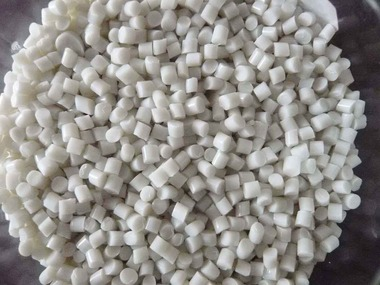
\includegraphics[width=0.4\textwidth]{images/PLA-Pellets.jpg}
        \caption{Pellets de PLA}
        \label{fig:Pellets de PLA}
    \end{figure}
    \item \textbf{Tolva:} depósito en el que cae la granza proveniente del dosificador. Debe proveer un flujo constante al extrusor para evitar cortes en el objeto que se está construyendo.
   
    Su diseño es muy importante, y en función del tipo de material que esté suministrando deberá ser de una manera u otra, debido a que el material puede llegar a compactarse en el fondo y no pasar a la extrusora. Algunos modelos de tolva incluyen sistemas de vibración para ayudar a que el material caiga. En la mayoría de los casos y dependiendo del material con el que estemos trabajando, será conveniente que incluya un sistema de secado para eliminar la humedad, puesto que dependiendo de la matería prima puede afectar a la hora de trabajar con el. Por ejemplo, con el uso del PLA es obligatorio su secado antes de la producción.
    \item \textbf{Cilindro hidráulico:} Constituye el cuerpo principal de la extrusora y en su interior está el husillo. Es en este cilindro donde se encuentran las resistencias electricas que aportan la energía calorífica necesaria para fundir el material. La temperatura está registrada a lo largo de las distintas zonas del cilindro, para poder tener un control sobre la temperatura de fusión del material. El cilindro debe estar fabricado con materiales especiales de tal manera, que tenga una buena transferencia de calor y debe ser más duro que el materíal que se está extruyendo, para lograr una larga duración.
    \item \textbf{Husillo:} Es el elemento más importante de la extrusora y el que determina el grado de calidad con el que la pieza saldrá de la extrusora.\\
            \begin{figure}[H]
                      \centering
                        \begin{subfigure}[b]{0.55\textwidth}
                                \centering
                            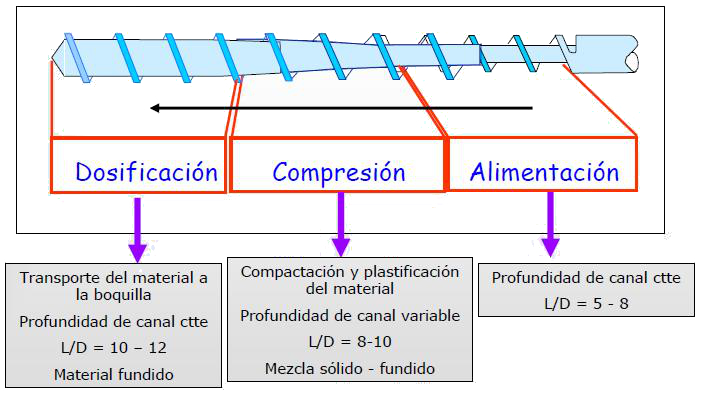
\includegraphics[width=\textwidth]{images/husillo.jpg}
                            \caption{Forma de un husillo. Fuente \cite{detallehusillo}}
                            \label{fig:estado_husillo1}
                        \end{subfigure}
                        
                        \begin{subfigure}[b]{0.55\textwidth}
                                \centering
                            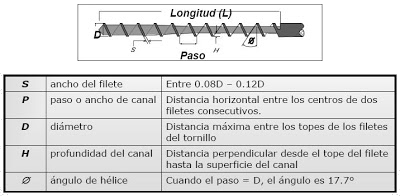
\includegraphics[width=\textwidth]{images/husillo2.jpg}
                            \caption{Parámetros de un husillo. Fuente  \cite{parametroshusillos}}
                            \label{fig:estado_husillo2}
                        \end{subfigure}
                        \caption{Características de un husillo.}
                        \label{fig:estado_husillo}
            \end{figure}
    Como se aprecia en la figura \ref{fig:estado_husillo1} tenemos tres zonas claramente definidas:
    \begin{itemize}
            \item \textbf{Alimentación:} Esta zona, es la encargada de transportar la granza de la tolva al interior del husillo. En la figura podemos ver como los filetes están muy separados del centro del husillo, con el fin de transportar la mayor cantidad posible de material.
            \item \textbf{Compresión:} A medida que entramos en la zona de compresión, los filetes van disminuyendo y se acercan al husillo, con el fin de fundir y homogeneizar el material. Aquí se expulsa el posible aire residual que quede entre la granza.
            \item \textbf{Dosificación:} Conduce el material compactado hacia el dado de la extrusora. Esta zona debe garantizar que el material sale con una temperatura constante y homogeneo.
    \end{itemize}
    \item \textbf{Dado:} En función del dado que se coloque al final de la extrusora, se conseguirá un perfil distinto, en el caso que nos ocupa, el dado tiene un círculo para conseguir la forma de cilindro que deseamos.
    \begin{figure}[H]
            \centering
            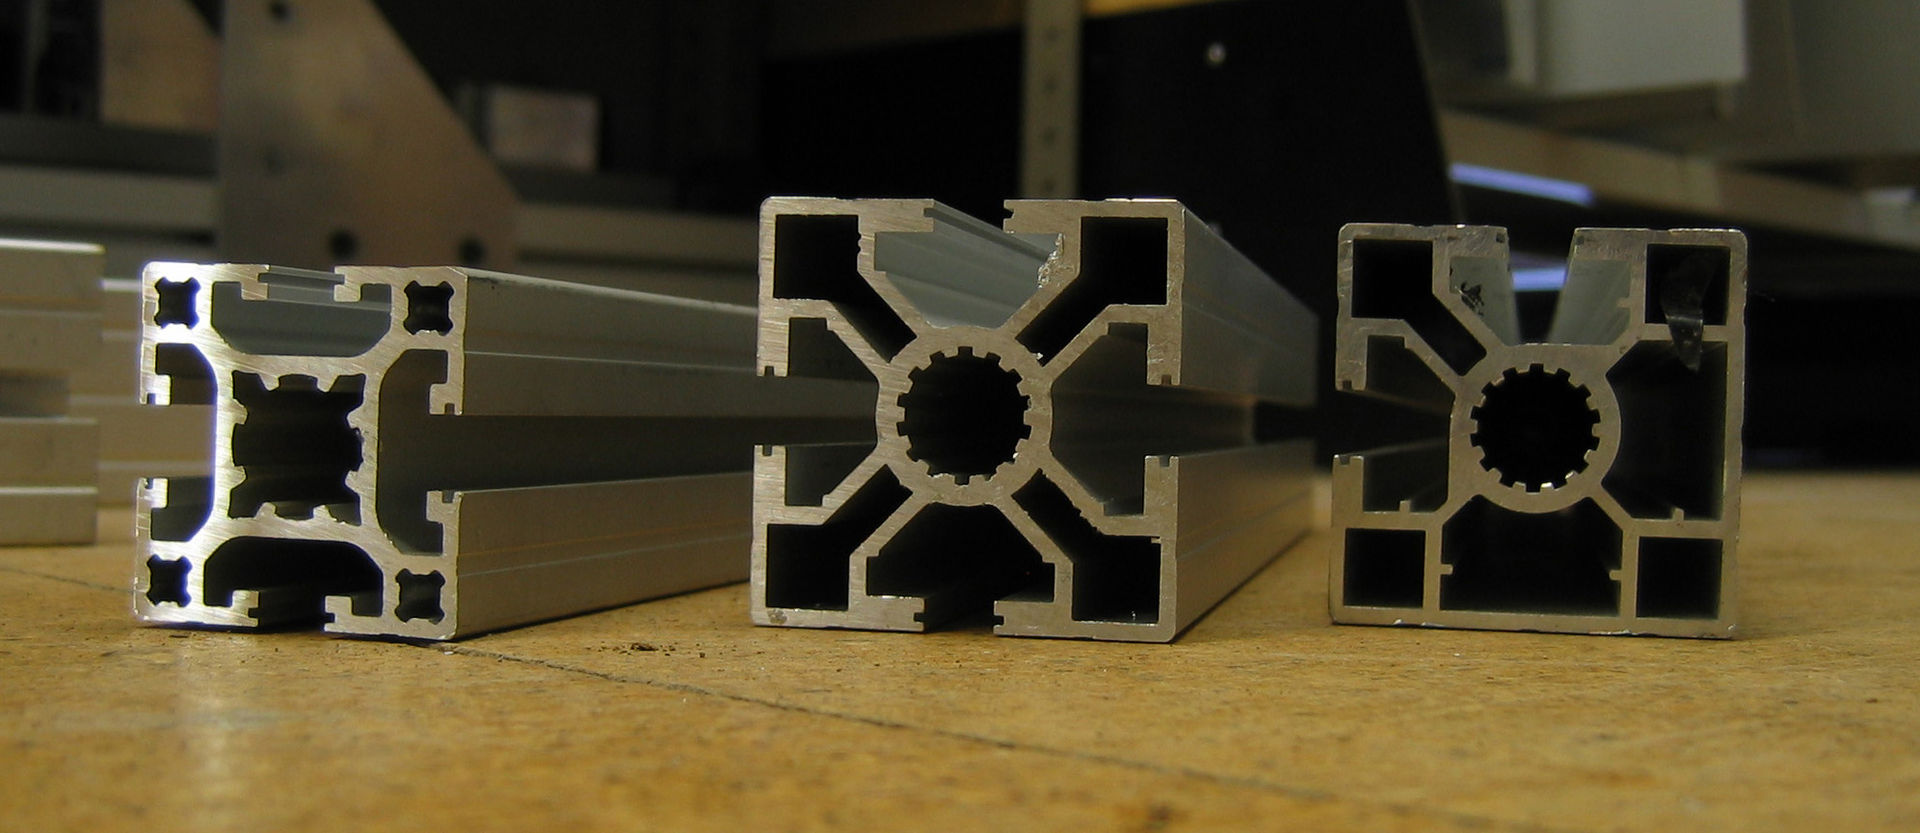
\includegraphics[width=0.5\textwidth]{images/Extruded_aluminium_section.jpg}
            \caption{Distintos ejemplos de extrusión. Fuente \cite{ejemplosextrusion}}
            \label{fig:estado_ejemplos}
    \end{figure}
\end{itemize}

\section{Fundamentos del control}
\label{arte_control}
\section{Comunicaciones industriales}
\label{arte_comunicaciones}
